%% Depiction of a marketing distribution channel or supply chain.
%% Author: Ashutosh Prasad
\documentclass{article}
\usepackage{tikz}
\usetikzlibrary{arrows,positioning}
\begin{document}

\begin{figure}
\centering
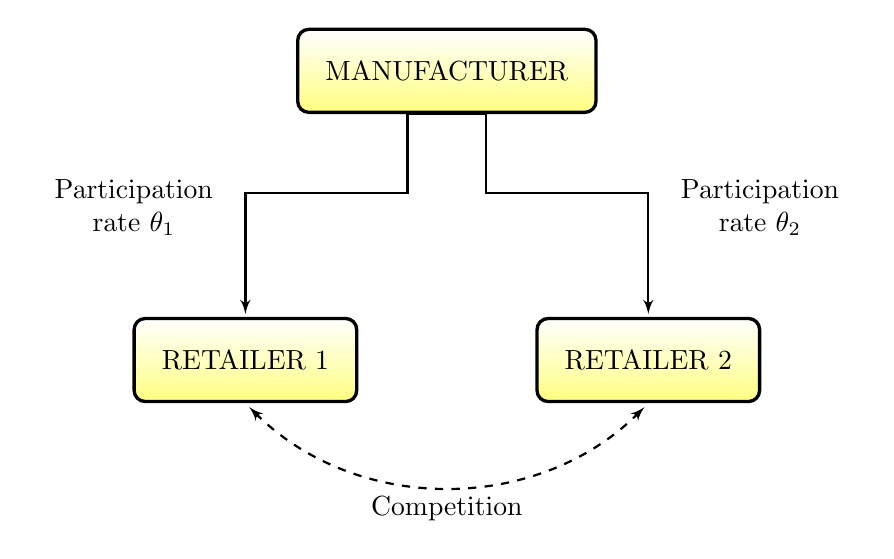
\begin{tikzpicture}[node distance=1cm, auto]
\tikzset{
    mynode/.style={rectangle,rounded corners,draw=black, top color=white, bottom color=yellow!50,very thick, inner sep=1em, minimum size=3em, text centered},
    myarrow/.style={->, >=latex', shorten >=1pt, thick},
    mylabel/.style={text width=7em, text centered}
}
\node[mynode] (manufacturer) {MANUFACTURER};
\node[below=3cm of manufacturer] (dummy) {};
\node[mynode, left=of dummy] (retailer1) {RETAILER 1};
\node[mynode, right=of dummy] (retailer2) {RETAILER 2};
\node[mylabel, below left=of manufacturer] (label1) {Participation rate $\theta_1$};
\node[mylabel, below right=of manufacturer] (label2) {Participation rate $\theta_2$};
% The text width of 7em forces the text to break into two lines.

\draw[myarrow] (manufacturer.south) -- ++(-.5,0) -- ++(0,-1) -|  (retailer1.north);
\draw[myarrow] (manufacturer.south) -- ++(.5,0) -- ++(0,-1) -|  (retailer2.north);
% There is a slight overlap of the arrows with the (manufacturer) south edge
% because creating the offset in another way didn't compile.

\draw[<->, >=latex', shorten >=2pt, shorten <=2pt, bend right=45, thick, dashed]
    (retailer1.south) to node[auto, swap] {Competition}(retailer2.south);
% The swap command corrects the placement of the text.

\end{tikzpicture}
\medskip
\caption{Structure of the Market}
\end{figure}

\end{document}
